\documentclass[notes,11pt, aspectratio=169]{beamer}

\usepackage{pgfpages}
\setbeameroption{hide notes}

\usepackage{helvet}
\usepackage[default]{lato}
\usepackage{array}
\usepackage{tgbonum}

\usepackage{tikz}
\usepackage{verbatim}
\setbeamertemplate{note page}{\pagecolor{yellow!5}\insertnote}
\usetikzlibrary{positioning}
\usetikzlibrary{calc}
\usetikzlibrary{arrows}
\usetikzlibrary{arrows.meta}
\usetikzlibrary{decorations.markings}
\usetikzlibrary{decorations.pathreplacing}
\usetikzlibrary{shapes.misc}
\usetikzlibrary{shapes.geometric}
\usetikzlibrary{matrix,shapes,arrows,fit,tikzmark}
\usepackage{amsmath}
\usepackage{amssymb}
\usepackage{mathtools}
\usepackage{bm}
\usepackage{mathpazo}
\usepackage{hyperref}
%\usepackage{lipsum}
%\usepackage{multimedia}
\usepackage{graphicx}
\usepackage{multirow}
\usepackage{dcolumn}
%\usepackage{bbm}   % PK-only fonts; not renderable by tectonic (indicator uses \mathbf{1})
\usepackage{pgfplots}
\pgfplotsset{compat=1.18}
\usepackage{listings}
\newcolumntype{d}[0]{D{.}{.}{5}}

\usepackage{changepage}
\usepackage{appendixnumberbeamer}
\newcommand{\beginbackup}{
   \newcounter{framenumbervorappendix}
   \setcounter{framenumbervorappendix}{\value{framenumber}}
   \setbeamertemplate{footline}
   {
     \leavevmode%
     \hline
     box{%
       \begin{beamercolorbox}[wd=\paperwidth,ht=2.25ex,dp=1ex,right]{footlinecolor}%
       \end{beamercolorbox}}%
     \vskip0pt%
   }
 }
\newcommand{\backupend}{
   \addtocounter{framenumbervorappendix}{-\value{framenumber}}
   \addtocounter{framenumber}{\value{framenumbervorappendix}}
}

\usepackage[space]{grffile}
\usepackage{booktabs}
\newcommand\independent{\protect\mathpalette{\protect\independenT}{\perp}}
\def\independenT#1#2{\mathrel{\rlap{$#1#2$}\mkern2mu{#1#2}}}
\DeclareMathOperator{\Supp}{Supp}
\DeclareMathOperator*{\argmin}{arg\,min}

\definecolor{blue}{RGB}{0,114,178}
\definecolor{red}{RGB}{213,94,0}
\definecolor{yellow}{RGB}{240,228,66}
\definecolor{green}{RGB}{0,158,115}

\hypersetup{
  colorlinks=true,
  linkbordercolor = {white},
  linkcolor = {blue}
}

\definecolor{MyBackground}{RGB}{255,253,218}

\newenvironment{transitionframe}{
  \setbeamercolor{background canvas}{bg=yellow}
  \begin{frame}}{
    \end{frame}
}

\setbeamercolor{frametitle}{fg=blue}
\setbeamercolor{title}{fg=black}
\setbeamertemplate{footline}[frame number]
\setbeamertemplate{navigation symbols}{}
\setbeamertemplate{itemize items}{-}
\setbeamercolor{itemize item}{fg=blue}
\setbeamercolor{itemize subitem}{fg=blue}
\setbeamercolor{enumerate item}{fg=blue}
\setbeamercolor{enumerate subitem}{fg=blue}
\setbeamercolor{button}{bg=MyBackground,fg=blue,}

\setbeamercolor{section in toc}{fg=blue}
\setbeamercolor{subsection in toc}{fg=red}
\setbeamersize{text margin left=1em,text margin right=1em}

\newenvironment{wideitemize}{\itemize\addtolength{\itemsep}{10pt}}{\enditemize}

\lstset{
    language=Python,
    basicstyle=\ttfamily\scriptsize,
    keywordstyle=\color{blue}\bfseries,
    stringstyle=\color{red!70!black},
    commentstyle=\color{green!50!black}\itshape,
    numbers=left,
    numberstyle=\tiny\color{gray},
    numbersep=5pt,
    frame=single,
    breaklines=true,
    backgroundcolor=\color{gray!5},
    showstringspaces=false,
    tabsize=4
}

\newcommand{\vx}{\mathbf{x}}
\newcommand{\vw}{\mathbf{w}}
\newcommand{\vb}{\mathbf{b}}
\newcommand{\vh}{\mathbf{h}}
\newcommand{\vy}{\mathbf{y}}
\newcommand{\vz}{\mathbf{z}}
\newcommand{\vc}{\mathbf{c}}
\newcommand{\vf}{\mathbf{f}}
\newcommand{\vi}{\mathbf{i}}
\newcommand{\vo}{\mathbf{o}}
\newcommand{\vr}{\mathbf{r}}
\newcommand{\vu}{\mathbf{u}}
\newcommand{\vW}{\mathbf{W}}
\newcommand{\vU}{\mathbf{U}}
\newcommand{\R}{\mathbb{R}}
\newcommand{\E}{\mathbb{E}}
\newcommand{\pd}[2]{\frac{\partial #1}{\partial #2}}


\title[]{\textcolor{blue}{Machine Learning II}\\ \textcolor{black}{\normalsize Lecture 3: Sequences: RNNs, LSTMs and GRUs}}
\author[Quispe]{}
\institute[ENEI]{\small{Alexander Quispe \\ ENEI -- INEI \,\textperiodcentered\, PEU-CD 2026}}
\date{October 12, 2026}


\begin{document}

\begin{frame}[plain]\titlepage\end{frame}

\begin{frame}{Outline}\tableofcontents\end{frame}


\tikzset{
        every picture/.style={remember picture,baseline},
        every node/.style={anchor=base,align=center,outer sep=1.5pt},
        every path/.style={thick},
        }
\tikzstyle{every picture}+=[remember picture]
\tikzstyle{mybox} =[draw=black, very thick, rectangle, inner sep=10pt, inner ysep=20pt]
\tikzstyle{fancytitle} =[draw=black,fill=red, text=white]




% ============================================================
\section{Recap and Motivation}
% ============================================================

\begin{transitionframe}
\begin{center}
{\Huge \textbf{Recap \& Motivation}}\\[10pt]
{\large Why do we need RNNs?}
\end{center}
\end{transitionframe}

\begin{frame}
\frametitle{Recap}

\textbf{What we learned about CNNs:}
\begin{itemize}
    \item \textbf{Inductive biases for images:} locality + translation invariance.
    \item \textbf{Convolution:} learn shared filters that slide across spatial dimensions.
    \item \textbf{Pooling:} downsample and accumulate receptive field.
    \item \textbf{Architectures:} LeNet $\to$ AlexNet $\to$ VGG $\to$ ResNet.
    \item Worked great for \textbf{images} (fixed-size, spatial structure).
\end{itemize}

\vspace{8pt}
\textbf{But what about \emph{sequential} data?}
\begin{center}
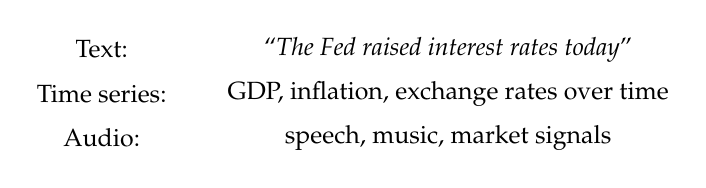
\begin{tikzpicture}[scale=0.8]
    \node[font=\small] at (0, 0) {Text:};
    \node[font=\small] at (5.5, 0) {``\textit{The Fed raised interest rates today}''};
    \node[font=\small] at (0, -0.7) {Time series:};
    \node[font=\small] at (5.5, -0.7) {GDP, inflation, exchange rates over time};
    \node[font=\small] at (0, -1.4) {Audio:};
    \node[font=\small] at (5.5, -1.4) {speech, music, market signals};
\end{tikzpicture}
\end{center}

\textcolor{red}{All have a \textbf{temporal/ordering} structure that CNNs don't naturally capture.}
\end{frame}

\begin{frame}
\frametitle{Why CNNs and MLPs Don't Work for Sequences}

\textbf{Three core challenges:}

\vspace{6pt}
\begin{enumerate}
    \item \textcolor{blue}{\textbf{Variable length:}} sentences have different numbers of words; time series have different histories. MLPs need a \textbf{fixed-size} input.

    \vspace{6pt}
    \item \textcolor{blue}{\textbf{Order matters:}} ``\textit{the cat ate the fish}'' $\neq$ ``\textit{the fish ate the cat}''. Bag-of-words representations lose all structure.

    \vspace{6pt}
    \item \textcolor{blue}{\textbf{Long-range dependencies:}} the meaning of a word may depend on something far back in the sentence. Inflation today depends on monetary policy years ago.
\end{enumerate}

\vspace{12pt}
\begin{tikzpicture}
\node [mybox] (box){%
    \begin{minipage}{0.93\textwidth}
    \vspace{-4pt}
    We need a model with \textbf{memory}: a state that summarizes what has been seen so far.
    \end{minipage}
};
\node[fancytitle, right=10pt] at (box.north west) {The Need for Memory};
\end{tikzpicture}
\end{frame}

\begin{frame}
\frametitle{Examples of Sequential Data in Economics}

\renewcommand{\arraystretch}{1.3}
\begin{center}
{\footnotesize
\begin{tabular}{p{3.8cm} p{5.5cm} p{4cm}}
\toprule
\textbf{Data type} & \textbf{Example} & \textbf{Task} \\
\midrule
Macro time series & GDP, CPI, unemployment & Forecasting, nowcasting \\
Financial time series & stock prices, FX rates, yields & Volatility, returns \\
Central bank text & FOMC minutes, ECB statements & Sentiment, policy class.\ \\
News articles & Bloomberg, Reuters headlines & Market reaction \\
Transaction data & credit card streams, payments & Fraud detection \\
Survey responses & sequential questions & Behavioral modeling \\
\bottomrule
\end{tabular}
}
\end{center}

\vspace{4pt}
\textbf{Common thread:} \textcolor{red}{order and timing carry information}.

RNNs (and later, Transformers) are the modern tools for these tasks.
\end{frame}


% ============================================================
\section{The RNN Idea: Adding Memory}
% ============================================================

\begin{transitionframe}
\begin{center}
{\Huge \textbf{The RNN Idea: Adding Memory}}
\end{center}
\end{transitionframe}

\begin{frame}
\frametitle{Core Idea: A Hidden State That Persists}

\textbf{Setup:} we receive inputs $\vx_1, \vx_2, \ldots, \vx_T$ one at a time.

\vspace{6pt}
\textbf{Idea:} at each step $t$, maintain a \textbf{hidden state} $\vh_t$ that summarizes everything seen so far.

\vspace{6pt}
\begin{tikzpicture}
\node [mybox] (box){%
    \begin{minipage}{0.93\textwidth}
    \vspace{-6pt}
    \[
        \vh_t = f(\vh_{t-1}, \vx_t)
    \]
    \vspace{-12pt}\\
    where $f$ is a learnable function (a small neural network).
    \end{minipage}
};
\node[fancytitle, right=10pt] at (box.north west) {The RNN Recurrence};
\end{tikzpicture}

\vspace{8pt}
\textbf{Properties:}
\begin{itemize}
    \item Same function $f$ applied at every time step (\textbf{parameter sharing}).
    \item Handles \textbf{variable-length} sequences naturally.
    \item State $\vh_t$ acts as memory of all past inputs $\vx_1, \ldots, \vx_t$.
\end{itemize}

\vspace{4pt}
\textcolor{red}{Parameter sharing across time is the temporal analogue of weight sharing in CNNs.}
\end{frame}

\begin{frame}
\frametitle{Rolled vs Unrolled View}

\begin{columns}[T]
\begin{column}{0.4\textwidth}
\centering
\textbf{Rolled (compact):}

\vspace{8pt}
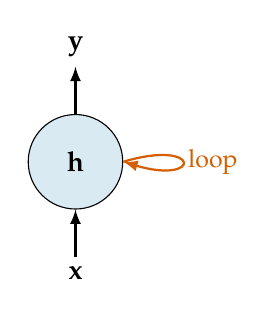
\begin{tikzpicture}[scale=1, >=latex]
    \node[draw, circle, fill=blue!15, minimum size=1.2cm] (h) at (0, 0) {$\vh$};
    \node[below=0.6cm of h] (x) {$\vx$};
    \node[above=0.6cm of h] (y) {$\vy$};
    \draw[->, thick] (x) -- (h);
    \draw[->, thick] (h) -- (y);
    % Self loop
    \draw[->, thick, red] (h.east) .. controls +(1,0.3) and +(1,-0.3) .. (h.east);
    \node[right=0.7cm of h, text=red, font=\small] {loop};
\end{tikzpicture}

\vspace{4pt}
{\small One block, with a self-loop.}
\end{column}

\begin{column}{0.55\textwidth}
\centering
\textbf{Unrolled (over time):}

\vspace{8pt}
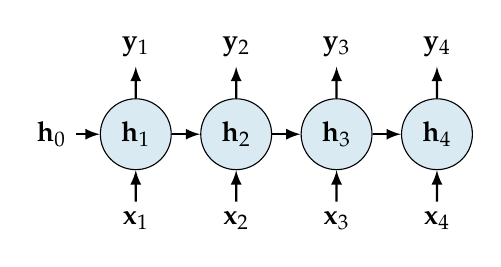
\begin{tikzpicture}[scale=0.85, >=latex]
    \foreach \t in {1,2,3,4} {
        \node[draw, circle, fill=blue!15, minimum size=0.9cm] (h\t) at (\t*1.5, 0) {$\vh_\t$};
        \node[below=0.4cm of h\t] (x\t) {$\vx_\t$};
        \node[above=0.4cm of h\t] (y\t) {$\vy_\t$};
        \draw[->, thick] (x\t) -- (h\t);
        \draw[->, thick] (h\t) -- (y\t);
    }
    \draw[->, thick] (h1) -- (h2);
    \draw[->, thick] (h2) -- (h3);
    \draw[->, thick] (h3) -- (h4);
    \node[left=0.3cm of h1] (h0) {$\vh_0$};
    \draw[->, thick] (h0) -- (h1);
\end{tikzpicture}

\vspace{4pt}
{\small Same network, replicated across $T$ time steps.}
\end{column}
\end{columns}

\vspace{12pt}
\textbf{Key insight:} the rolled and unrolled views are \textbf{equivalent}. The unrolled view makes backpropagation conceptually clear.

\textcolor{red}{All time steps share the same parameters.}
\end{frame}


% ============================================================
\section{Vanilla RNN Architecture and Math}
% ============================================================

\begin{transitionframe}
\begin{center}
{\Huge \textbf{Vanilla RNN: Architecture \& Math}}
\end{center}
\end{transitionframe}

\begin{frame}
\frametitle{The Vanilla RNN Equations}

\begin{tikzpicture}
\node [mybox] (box){%
    \begin{minipage}{0.93\textwidth}
    \vspace{-6pt}
    \textbf{Hidden state} (the recurrence):
    \[
        \vh_t = \tanh(\vW_{hh} \vh_{t-1} + \vW_{xh} \vx_t + \vb_h)
    \]

    \textbf{Output} (the prediction at time $t$):
    \[
        \vy_t = \vW_{hy} \vh_t + \vb_y
    \]
    \vspace{-12pt}
    \end{minipage}
};
\node[fancytitle, right=10pt] at (box.north west) {Vanilla RNN};
\end{tikzpicture}

\vspace{8pt}
\textbf{Dimensions:} let $d$ = input size, $h$ = hidden size, $k$ = output size.
\begin{itemize}
    \item $\vx_t \in \R^d$, \; $\vh_t \in \R^h$, \; $\vy_t \in \R^k$
    \item $\vW_{xh} \in \R^{h \times d}$, \; $\vW_{hh} \in \R^{h \times h}$ (recurrent), \; $\vW_{hy} \in \R^{k \times h}$
\end{itemize}

\vspace{4pt}
\textbf{Total parameters:} $hd + h^2 + kh + h + k$ --- \textcolor{red}{independent of sequence length $T$}.
\end{frame}

\begin{frame}
\frametitle{Unrolled Computational Graph}

\begin{center}
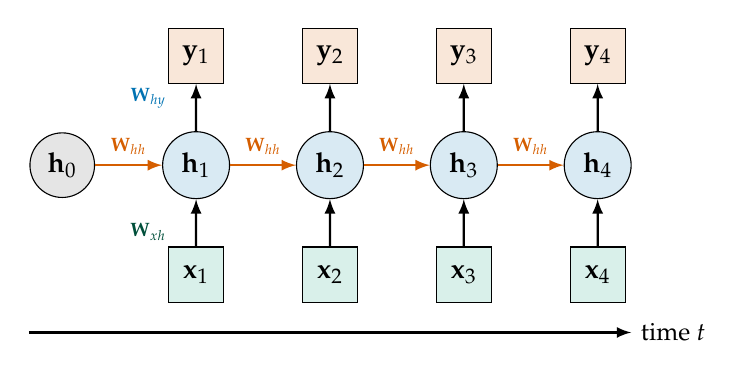
\begin{tikzpicture}[scale=0.85, >=latex]
    % Initial hidden state
    \node[draw, circle, fill=gray!20, minimum size=0.7cm] (h0) at (0, 0) {$\vh_0$};

    \foreach \t in {1,2,3,4} {
        % Hidden states
        \node[draw, circle, fill=blue!15, minimum size=0.85cm] (h\t) at (\t*2, 0) {$\vh_\t$};
        % Inputs
        \node[draw, fill=green!15, minimum size=0.7cm, below=0.6cm of h\t] (x\t) {$\vx_\t$};
        % Outputs
        \node[draw, fill=red!15, minimum size=0.7cm, above=0.6cm of h\t] (y\t) {$\vy_\t$};
        % Connections
        \draw[->, thick] (x\t) -- (h\t);
        \draw[->, thick] (h\t) -- (y\t);
    }

    % Recurrent connections
    \draw[->, thick, red] (h0) -- node[above, font=\scriptsize] {$\vW_{hh}$} (h1);
    \draw[->, thick, red] (h1) -- node[above, font=\scriptsize] {$\vW_{hh}$} (h2);
    \draw[->, thick, red] (h2) -- node[above, font=\scriptsize] {$\vW_{hh}$} (h3);
    \draw[->, thick, red] (h3) -- node[above, font=\scriptsize] {$\vW_{hh}$} (h4);

    % Input/output weight labels
    \node[left, font=\scriptsize, text=green!50!black] at (1.7, -1) {$\vW_{xh}$};
    \node[left, font=\scriptsize, text=blue] at (1.7, 1) {$\vW_{hy}$};

    % Time axis
    \draw[->, thick] (-0.5, -2.5) -- (8.5, -2.5);
    \node[right, font=\small] at (8.5, -2.5) {time $t$};
\end{tikzpicture}
\end{center}

\vspace{6pt}
\textbf{Each time step uses the \emph{same} weights} ($\vW_{xh}, \vW_{hh}, \vW_{hy}$). Information flows forward through the red recurrent connections.
\end{frame}

\begin{frame}
\frametitle{Numerical Example: Forward Pass}

\textbf{Tiny RNN:} $d = 1$, $h = 2$, $k = 1$. Inputs: $\vx_1 = 1, \vx_2 = 2, \vx_3 = 3$.

\vspace{4pt}
\textbf{Parameters:}
\[
    \vW_{xh} = \begin{pmatrix} 0.5 \\ 0.3 \end{pmatrix},\quad
    \vW_{hh} = \begin{pmatrix} 0.1 & 0.2 \\ 0.3 & 0.4 \end{pmatrix},\quad
    \vW_{hy} = \begin{pmatrix} 0.2 & 0.5 \end{pmatrix},\quad
    \vb_h = \mathbf{0},\ \vb_y = 0
\]

\textbf{Initial state:} $\vh_0 = \mathbf{0}$.

\vspace{4pt}
\textbf{Time $t = 1$:}
\[
    \vh_1 = \tanh(\vW_{hh} \cdot \mathbf{0} + \vW_{xh} \cdot 1) = \tanh\!\begin{pmatrix}0.5\\0.3\end{pmatrix} \approx \begin{pmatrix}0.462\\0.291\end{pmatrix}
\]

\textbf{Time $t = 2$:}
\[
    \vh_2 = \tanh\!\left(\begin{pmatrix}0.1 & 0.2\\0.3 & 0.4\end{pmatrix}\!\begin{pmatrix}0.462\\0.291\end{pmatrix} + \begin{pmatrix}0.5\\0.3\end{pmatrix}\!\cdot 2\right) \approx \begin{pmatrix}0.847\\0.946\end{pmatrix}
\]

\textbf{Output at $t = 2$:} $y_2 = 0.2 \cdot 0.847 + 0.5 \cdot 0.946 = \textcolor{red}{0.642}$.
\end{frame}

\begin{frame}
\frametitle{RNN Architectures (Karpathy's Diagram)}

\begin{center}
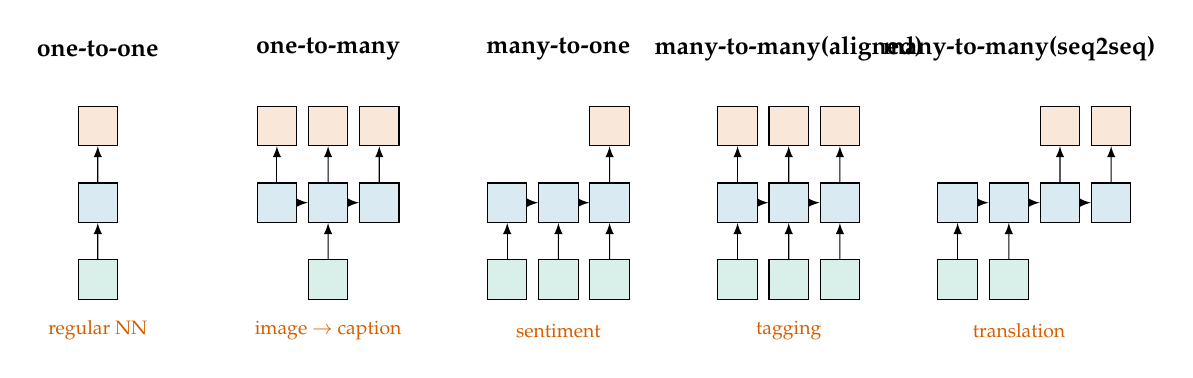
\begin{tikzpicture}[scale=0.65, >=latex]
\foreach \shift/\nin/\nout/\name/\example in {
    0/1/1/{one-to-one}/{regular NN},
    4.5/1/3/{one-to-many}/{image $\to$ caption},
    9/3/1/{many-to-one}/{sentiment},
    13.5/3/3/{many-to-many\\(aligned)}/{tagging},
    18/3/3/{many-to-many\\(seq2seq)}/{translation}
} {
    \begin{scope}[xshift=\shift cm]
        \node[font=\bfseries\small] at (1.5, 4.5) {\name};
        \node[font=\scriptsize, text=red] at (1.5, -1) {\example};
    \end{scope}
}

% --- one-to-one ---
\begin{scope}[xshift=0cm]
    \node[draw, fill=green!15, minimum size=0.5cm] (xa) at (1.5, 0) {};
    \node[draw, fill=blue!15, minimum size=0.5cm] (ha) at (1.5, 1.5) {};
    \node[draw, fill=red!15, minimum size=0.5cm] (ya) at (1.5, 3) {};
    \draw[->] (xa) -- (ha);
    \draw[->] (ha) -- (ya);
\end{scope}

% --- one-to-many ---
\begin{scope}[xshift=4.5cm]
    \node[draw, fill=green!15, minimum size=0.5cm] (xb) at (1.5, 0) {};
    \foreach \i in {0,1,2} {
        \node[draw, fill=blue!15, minimum size=0.5cm] (hb\i) at (\i+0.5, 1.5) {};
        \node[draw, fill=red!15, minimum size=0.5cm] (yb\i) at (\i+0.5, 3) {};
        \draw[->] (hb\i) -- (yb\i);
    }
    \draw[->] (xb) -- (hb1);
    \draw[->] (hb0) -- (hb1);
    \draw[->] (hb1) -- (hb2);
\end{scope}

% --- many-to-one ---
\begin{scope}[xshift=9cm]
    \node[draw, fill=red!15, minimum size=0.5cm] (yc) at (2.5, 3) {};
    \foreach \i in {0,1,2} {
        \node[draw, fill=green!15, minimum size=0.5cm] (xc\i) at (\i+0.5, 0) {};
        \node[draw, fill=blue!15, minimum size=0.5cm] (hc\i) at (\i+0.5, 1.5) {};
        \draw[->] (xc\i) -- (hc\i);
    }
    \draw[->] (hc0) -- (hc1);
    \draw[->] (hc1) -- (hc2);
    \draw[->] (hc2) -- (yc);
\end{scope}

% --- many-to-many aligned ---
\begin{scope}[xshift=13.5cm]
    \foreach \i in {0,1,2} {
        \node[draw, fill=green!15, minimum size=0.5cm] (xd\i) at (\i+0.5, 0) {};
        \node[draw, fill=blue!15, minimum size=0.5cm] (hd\i) at (\i+0.5, 1.5) {};
        \node[draw, fill=red!15, minimum size=0.5cm] (yd\i) at (\i+0.5, 3) {};
        \draw[->] (xd\i) -- (hd\i);
        \draw[->] (hd\i) -- (yd\i);
    }
    \draw[->] (hd0) -- (hd1);
    \draw[->] (hd1) -- (hd2);
\end{scope}

% --- many-to-many seq2seq ---
\begin{scope}[xshift=18cm]
    \foreach \i in {0,1} {
        \node[draw, fill=green!15, minimum size=0.5cm] (xe\i) at (\i+0.3, 0) {};
        \node[draw, fill=blue!15, minimum size=0.5cm] (he\i) at (\i+0.3, 1.5) {};
        \draw[->] (xe\i) -- (he\i);
    }
    \foreach \i in {2,3} {
        \node[draw, fill=blue!15, minimum size=0.5cm] (he\i) at (\i+0.3, 1.5) {};
        \node[draw, fill=red!15, minimum size=0.5cm] (ye\i) at (\i+0.3, 3) {};
        \draw[->] (he\i) -- (ye\i);
    }
    \draw[->] (he0) -- (he1);
    \draw[->] (he1) -- (he2);
    \draw[->] (he2) -- (he3);
\end{scope}
\end{tikzpicture}
\end{center}

\vspace{6pt}
{\small \textcolor{blue}{Hidden states (blue)}, \textcolor{green!50!black}{inputs (green)}, \textcolor{red}{outputs (red)}.}
\end{frame}


% ============================================================
\section{Backpropagation Through Time}
% ============================================================

\begin{transitionframe}
\begin{center}
{\Huge \textbf{Backpropagation Through Time (BPTT)}}
\end{center}
\end{transitionframe}

\begin{frame}
\frametitle{The Loss and Gradient Goal}

For a sequence with predictions $\vy_1, \ldots, \vy_T$ and targets $\hat\vy_1, \ldots, \hat\vy_T$:
\[
    \mathcal{L} = \sum_{t=1}^{T} \mathcal{L}_t(\vy_t, \hat\vy_t)
\]

\vspace{6pt}
\textbf{Goal:} compute $\pd{\mathcal{L}}{\vW_{hh}}, \pd{\mathcal{L}}{\vW_{xh}}, \pd{\mathcal{L}}{\vW_{hy}}$ to update the weights.

\vspace{8pt}
\textbf{Challenge:} $\vW_{hh}$ is used \textbf{at every time step}. So:
\[
    \pd{\mathcal{L}}{\vW_{hh}} = \sum_{t=1}^{T} \pd{\mathcal{L}_t}{\vW_{hh}}
\]

\vspace{4pt}
And each $\mathcal{L}_t$ depends on $\vW_{hh}$ through \textbf{all} hidden states $\vh_1, \ldots, \vh_t$.

\vspace{4pt}
\textcolor{red}{This is just the chain rule applied to the unrolled graph: backpropagation through time.}
\end{frame}

\begin{frame}
\frametitle{BPTT: The Chain Rule Through Time}

For a single loss $\mathcal{L}_t$ at time $t$, the gradient w.r.t.\ $\vW_{hh}$ involves \textbf{all earlier hidden states}:

\vspace{6pt}
\begin{tikzpicture}
\node [mybox] (box){%
    \begin{minipage}{0.93\textwidth}
    \vspace{-6pt}
    \[
        \pd{\mathcal{L}_t}{\vW_{hh}} = \sum_{k=1}^{t} \pd{\mathcal{L}_t}{\vh_t} \cdot \pd{\vh_t}{\vh_k} \cdot \pd{\vh_k}{\vW_{hh}}
    \]

    where the \textcolor{red}{\textbf{Jacobian product}} is:
    \[
        \pd{\vh_t}{\vh_k} = \prod_{i=k+1}^{t} \pd{\vh_i}{\vh_{i-1}} = \prod_{i=k+1}^{t} \vW_{hh}^\top \, \mathrm{diag}(\tanh'(\vz_i))
    \]
    where $\vz_i = \vW_{hh} \vh_{i-1} + \vW_{xh} \vx_i + \vb_h$.
    \end{minipage}
};
\node[fancytitle, right=10pt] at (box.north west) {BPTT Formula};
\end{tikzpicture}

\vspace{4pt}
The gradient flowing back from $t$ to $k$ is a \textbf{product of $t-k$ Jacobians}.

\textcolor{red}{This product is the source of vanishing/exploding gradients.}
\end{frame}

\begin{frame}
\frametitle{Truncated BPTT (Practical Trick)}

\textbf{Problem:} for long sequences (e.g., 1000 tokens), backprop through all $T$ steps is expensive and unstable.

\vspace{6pt}
\textbf{Solution:} \textbf{truncated BPTT} -- only backpropagate through the last $K$ steps (e.g., $K = 35$ or $K = 100$).

\vspace{8pt}
\begin{center}
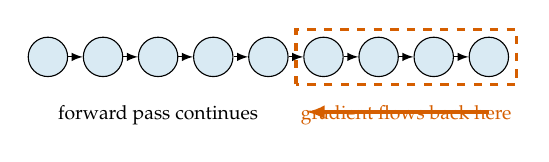
\begin{tikzpicture}[scale=0.7, >=latex]
    \foreach \t in {1,...,9} {
        \node[draw, circle, fill=blue!15, minimum size=0.5cm] (h\t) at (\t, 0) {};
    }
    \foreach \t in {1,...,8} {
        \pgfmathtruncatemacro{\next}{\t+1}
        \draw[->] (h\t) -- (h\next);
    }

    % Highlight the last K steps
    \draw[red, very thick, dashed] (5.5, -0.5) rectangle (9.5, 0.5);
    \node[below, font=\scriptsize, text=red] at (7.5, -0.7) {gradient flows back here};
    \node[below, font=\scriptsize] at (3, -0.7) {forward pass continues};

    % Truncation marker
    \draw[->, very thick, red] (9, -1) -- (5.7, -1);
\end{tikzpicture}
\end{center}

\vspace{6pt}
\textbf{Trade-off:} can't learn dependencies longer than $K$ steps, but training is feasible.

\vspace{4pt}
\textbf{In PyTorch:} use \texttt{detach()} on the hidden state every $K$ steps.
\end{frame}


% ============================================================
\section{The Vanishing Gradient Problem}
% ============================================================

\begin{transitionframe}
\begin{center}
{\Huge \textbf{The Vanishing/Exploding Gradient Problem}}
\end{center}
\end{transitionframe}

\begin{frame}
\frametitle{Why Long-Range Dependencies Are Hard}

Recall the gradient flowing from time $t$ back to time $k$:
\[
    \pd{\vh_t}{\vh_k} = \prod_{i=k+1}^{t} \vW_{hh}^\top \, \mathrm{diag}(\tanh'(\vz_i))
\]

\vspace{4pt}
\textbf{Two facts:}
\begin{wideitemize}
    \item $\tanh'(z) \in [0, 1]$, with maximum at $z = 0$.
    \item Multiplying many matrices $\vW_{hh}^\top$ together $\Rightarrow$ behavior governed by the \textbf{spectral radius} (largest eigenvalue magnitude) $\rho(\vW_{hh})$.
\end{wideitemize}

\vspace{8pt}
\begin{tikzpicture}
\node [mybox] (box){%
    \begin{minipage}{0.93\textwidth}
    \vspace{-4pt}
    \begin{itemize}
        \item If $\rho(\vW_{hh}) < 1$: gradient \textcolor{red}{\textbf{vanishes}} exponentially $\to 0$.
        \item If $\rho(\vW_{hh}) > 1$: gradient \textcolor{red}{\textbf{explodes}} exponentially $\to \infty$.
    \end{itemize}
    \end{minipage}
};
\node[fancytitle, right=10pt] at (box.north west) {Spectral Analysis};
\end{tikzpicture}
\end{frame}

\begin{frame}{Vanishing Gradients: The Product of Jacobians}\footnotesize
For $\mathbf{h}_t=\sigma(\mathbf{W}\mathbf{h}_{t-1}+\mathbf{U}\mathbf{x}_t+\mathbf{b})$, write $\mathbf{a}_t=\mathbf{W}\mathbf{h}_{t-1}+\mathbf{U}\mathbf{x}_t+\mathbf{b}$.
\begin{block}{One step of the chain rule}
\[
\frac{\partial\mathbf{h}_t}{\partial\mathbf{h}_{t-1}}=\operatorname{diag}\!\bigl(\sigma'(\mathbf{a}_t)\bigr)\,\mathbf{W},
\qquad\text{so}\qquad
\frac{\partial\mathbf{h}_T}{\partial\mathbf{h}_t}=\prod_{k=t+1}^{T}\operatorname{diag}\!\bigl(\sigma'(\mathbf{a}_k)\bigr)\,\mathbf{W}.
\]
\end{block}
\begin{block}{Bounding the product}
Let $\gamma=\max_z\sigma'(z)$ ($\gamma=1$ for $\tanh$, $\gamma=\tfrac14$ for the sigmoid) and $\|\mathbf{W}\|_2$ the largest singular value. Sub-multiplicativity of the spectral norm gives
\[
\Bigl\|\frac{\partial\mathbf{h}_T}{\partial\mathbf{h}_t}\Bigr\|_2\ \le\ \prod_{k=t+1}^{T}\bigl\|\operatorname{diag}(\sigma'(\mathbf{a}_k))\bigr\|_2\,\|\mathbf{W}\|_2\ \le\ \bigl(\gamma\,\|\mathbf{W}\|_2\bigr)^{\,T-t}.
\]
\end{block}
\begin{itemize}
  \item If $\gamma\|\mathbf{W}\|_2<1$ the bound decays \textbf{exponentially} in the time gap $T-t$: the gradient from a loss at time $T$ cannot reach a parameter that mattered at time $t$. This is the vanishing-gradient problem, and it is unavoidable for a sigmoid ($\gamma=\tfrac14$) unless $\|\mathbf{W}\|_2>4$.
  \item If $\gamma\|\mathbf{W}\|_2>1$ nothing prevents \textbf{explosion}; gradient clipping is the standard patch.
  \item The LSTM's cell state has Jacobian $\operatorname{diag}(\mathbf{f}_t)$ --- the forget gate --- with no $\mathbf{W}$ in the product. That is the whole design.
\end{itemize}
\end{frame}

\begin{frame}
\frametitle{Visualizing Vanishing Gradients}

\textbf{Setting:} $\vW_{hh}$ scalar with $w \in \{0.5, 0.9, 1.0, 1.1\}$ (1D RNN, $\tanh' \approx 1$).

\begin{center}
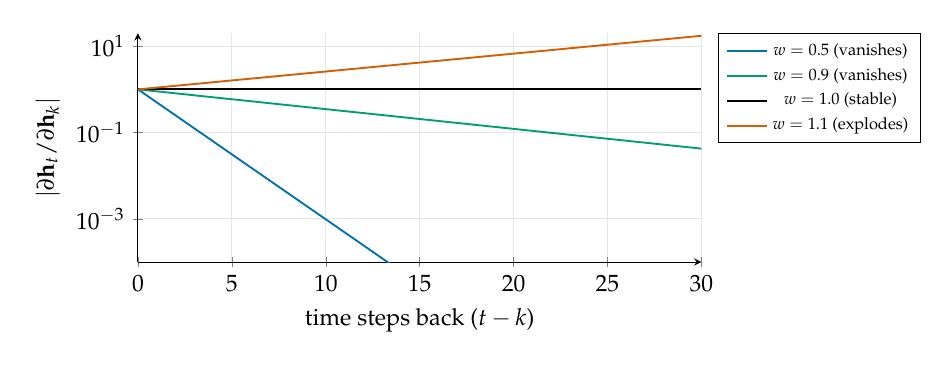
\begin{tikzpicture}[scale=0.85]
    \begin{axis}[
        xlabel={time steps back ($t-k$)}, ylabel={$|\partial \vh_t / \partial \vh_k|$},
        xmin=0, xmax=30, ymin=0.0001, ymax=20,
        ymode=log,
        width=10cm, height=5cm,
        axis lines=left,
        legend pos=outer north east,
        legend style={font=\scriptsize},
        grid=major, grid style={gray!20}
    ]
    \addplot[thick, blue, domain=0:30, samples=31] {0.5^x};
    \addlegendentry{$w=0.5$ (vanishes)}
    \addplot[thick, green, domain=0:30, samples=31] {0.9^x};
    \addlegendentry{$w=0.9$ (vanishes)}
    \addplot[thick, black, domain=0:30, samples=31] {1.0^x};
    \addlegendentry{$w=1.0$ (stable)}
    \addplot[thick, red, domain=0:30, samples=31] {1.1^x};
    \addlegendentry{$w=1.1$ (explodes)}
    \end{axis}
\end{tikzpicture}
\end{center}

\vspace{6pt}
\textbf{Practical consequence:} vanilla RNNs cannot learn dependencies more than \textbf{$\approx$10--20 time steps} apart.

\textcolor{red}{This is a fundamental limitation, not a training issue.}
\end{frame}

\begin{frame}
\frametitle{Partial Fixes (Insufficient)}

\textbf{Gradient clipping} (for exploding gradients):
\[
    \text{if } \|\nabla\| > c, \quad \nabla \leftarrow \frac{c}{\|\nabla\|} \nabla
\]
Caps gradient magnitude. Helps with explosion, \emph{not} with vanishing.

\vspace{8pt}
\textbf{Initialization:} initialize $\vW_{hh}$ as orthogonal or identity matrix. Helps at the start, but breaks down during training.

\vspace{8pt}
\textbf{ReLU instead of tanh:} doesn't saturate, but introduces other instabilities.

\vspace{12pt}
\begin{center}
\fbox{\textbf{None of these solve the fundamental problem.}}
\end{center}

\vspace{4pt}
\begin{center}
\textcolor{red}{We need a fundamentally different architecture: \textbf{LSTM}.}
\end{center}
\end{frame}


% ============================================================
\section{LSTM: The Solution}
% ============================================================

\begin{transitionframe}
\begin{center}
{\Huge \textbf{Long Short-Term Memory (LSTM)}}\\[10pt]
{\large Hochreiter \& Schmidhuber (1997)}
\end{center}
\end{transitionframe}

\begin{frame}
\frametitle{LSTM: The Key Idea}

\textbf{Vanilla RNN problem:} information must squeeze through the recurrent path at every step. Repeated multiplications destroy gradients.

\vspace{6pt}
\textbf{LSTM solution:} introduce a separate \textbf{cell state} $\vc_t$ that flows through time \emph{additively}, with \textbf{gates} that control information flow.

\vspace{6pt}
\begin{center}
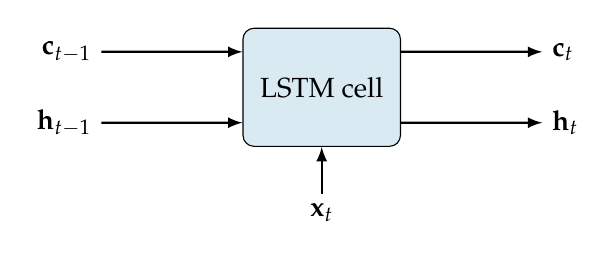
\begin{tikzpicture}[>=latex, scale=0.9]
    \node[draw, rounded corners, fill=blue!15, minimum width=2cm, minimum height=1.5cm] (lstm) at (0, 0) {LSTM cell};

    % Inputs
    \node[left=1cm of lstm] (cin) at (-2, 0.5) {$\vc_{t-1}$};
    \node[left=1cm of lstm] (hin) at (-2, -0.5) {$\vh_{t-1}$};
    \node[below=0.6cm of lstm] (xin) {$\vx_t$};

    % Outputs
    \node[right=1cm of lstm] (cout) at (2, 0.5) {$\vc_t$};
    \node[right=1cm of lstm] (hout) at (2, -0.5) {$\vh_t$};

    \draw[->, thick] (cin) -- ([yshift=0.5cm]lstm.west);
    \draw[->, thick] (hin) -- ([yshift=-0.5cm]lstm.west);
    \draw[->, thick] (xin) -- (lstm.south);
    \draw[->, thick] ([yshift=0.5cm]lstm.east) -- (cout);
    \draw[->, thick] ([yshift=-0.5cm]lstm.east) -- (hout);
\end{tikzpicture}
\end{center}

\vspace{6pt}
\textbf{Two memory streams:}
\begin{itemize}
    \item \textbf{Cell state} $\vc_t$: the ``long-term'' memory (highway for gradients).
    \item \textbf{Hidden state} $\vh_t$: the ``working memory'' / output for this time step.
\end{itemize}
\end{frame}

\begin{frame}
\frametitle{The Three Gates}

A gate is a vector in $[0,1]^h$ from a sigmoid. Element-wise multiplication acts as a soft mask: 0 = ``forget'', 1 = ``keep''.

\vspace{4pt}
\textbf{Forget gate} (what to drop from $\vc_{t-1}$):
\[
    \vf_t = \sigma(\vW_f [\vh_{t-1}, \vx_t] + \vb_f)
\]

\textbf{Input gate} (what new info to add):
\[
    \vi_t = \sigma(\vW_i [\vh_{t-1}, \vx_t] + \vb_i)
\]

\textbf{Output gate} (what part of $\vc_t$ to expose as $\vh_t$):
\[
    \vo_t = \sigma(\vW_o [\vh_{t-1}, \vx_t] + \vb_o)
\]

\textbf{Candidate value} (proposed new info):
\[
    \tilde\vc_t = \tanh(\vW_c [\vh_{t-1}, \vx_t] + \vb_c)
\]

{\small $[\vh_{t-1}, \vx_t]$ = concatenation, so $\vW_f \in \R^{h \times (h+d)}$.}
\end{frame}

\begin{frame}
\frametitle{The LSTM Updates}

Putting it all together:

\vspace{6pt}
\begin{tikzpicture}
\node [mybox] (box){%
    \begin{minipage}{0.93\textwidth}
    \vspace{-4pt}
    \textbf{Cell state update:}
    \[
        \vc_t = \vf_t \odot \vc_{t-1} + \vi_t \odot \tilde\vc_t
    \]

    \textbf{Hidden state:}
    \[
        \vh_t = \vo_t \odot \tanh(\vc_t)
    \]
    \vspace{-12pt}
    \end{minipage}
};
\node[fancytitle, right=10pt] at (box.north west) {LSTM Updates};
\end{tikzpicture}

\vspace{4pt}
\textbf{Reading the cell state:} keep $\vf_t \odot \vc_{t-1}$ from old memory, add $\vi_t \odot \tilde\vc_t$ new info. The \textbf{additive} update is key to gradient flow.

\textbf{Reading the hidden state:} cell state squashed by $\tanh$, then masked by output gate.
\end{frame}

\begin{frame}
\frametitle{LSTM Cell: Visual Diagram}

\begin{center}
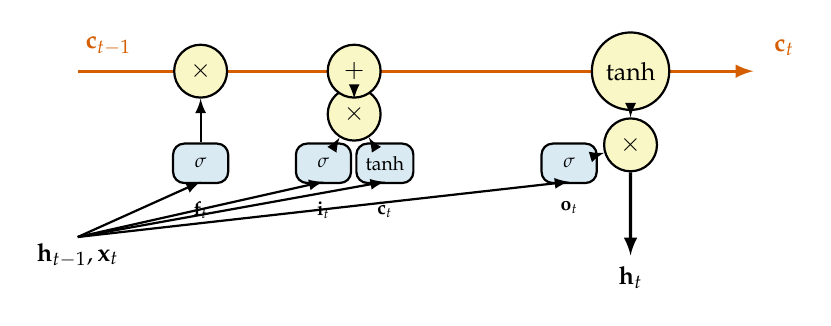
\begin{tikzpicture}[scale=0.78, >=latex,
    op/.style={circle, draw, thick, fill=yellow!30, minimum size=0.5cm, font=\small},
    gate/.style={rectangle, draw, thick, rounded corners, fill=blue!15, minimum width=0.7cm, minimum height=0.5cm, font=\scriptsize}]

    % Cell state highway (top)
    \draw[->, very thick, red] (-1, 3) -- (10, 3);
    \node[font=\small, text=red, above] at (-0.5, 3.1) {$\vc_{t-1}$};
    \node[font=\small, text=red, above] at (10.5, 3.1) {$\vc_t$};

    % Forget gate
    \node[gate] (f) at (1, 1.5) {$\sigma$};
    \node[op] (mult1) at (1, 3) {$\times$};
    \draw[->, thick] (f) -- (mult1);
    \node[below=0.1cm of f, font=\scriptsize] {$\vf_t$};

    % Input gate
    \node[gate] (i) at (3, 1.5) {$\sigma$};
    \node[gate] (cand) at (4, 1.5) {tanh};
    \node[op] (mult2) at (3.5, 2.3) {$\times$};
    \node[op] (plus) at (3.5, 3) {$+$};
    \draw[->, thick] (i) -- (mult2);
    \draw[->, thick] (cand) -- (mult2);
    \draw[->, thick] (mult2) -- (plus);
    \node[below=0.1cm of i, font=\scriptsize] {$\vi_t$};
    \node[below=0.1cm of cand, font=\scriptsize] {$\tilde\vc_t$};

    % Output gate
    \node[gate] (o) at (7, 1.5) {$\sigma$};
    \node[op] (tanhc) at (8, 3) {tanh};
    \node[op] (mult3) at (8, 1.8) {$\times$};
    \draw[->, thick] (tanhc) -- (mult3);
    \draw[->, thick] (o) -- (mult3);
    \node[below=0.1cm of o, font=\scriptsize] {$\vo_t$};

    % Hidden state output
    \draw[->, very thick] (mult3) -- (8, 0) node[below, font=\small] {$\vh_t$};

    % Inputs at bottom
    \node[font=\small] at (-1, 0) {$\vh_{t-1}, \vx_t$};
    \draw[thick, ->] (-1, 0.3) -- (1, 1.2);
    \draw[thick, ->] (-1, 0.3) -- (3, 1.2);
    \draw[thick, ->] (-1, 0.3) -- (4, 1.2);
    \draw[thick, ->] (-1, 0.3) -- (7, 1.2);
\end{tikzpicture}
\end{center}

\vspace{4pt}
\textbf{Red highway:} cell state path. \textbf{Yellow circles:} pointwise operations. \textbf{Blue boxes:} learned gates.
\end{frame}

\begin{frame}
\frametitle{Why LSTMs Solve Vanishing Gradients}

\textbf{Gradient flow through the cell state:}
\[
    \pd{\vc_t}{\vc_{t-1}} = \mathrm{diag}(\vf_t)
\]

\textbf{Compare with vanilla RNN:}
\[
    \pd{\vh_t}{\vh_{t-1}} = \vW_{hh}^\top \, \mathrm{diag}(\tanh'(\vz_t))
\]

\vspace{4pt}
\begin{tikzpicture}
\node [mybox] (box){%
    \begin{minipage}{0.93\textwidth}
    \vspace{-4pt}
    \textbf{Key difference:} LSTM gradient is just $\vf_t$. If the network learns $\vf_t \approx 1$ for relevant steps, gradient flows back \textbf{intact} through arbitrarily many time steps.
    \end{minipage}
};
\node[fancytitle, right=10pt] at (box.north west) {The Crucial Insight};
\end{tikzpicture}

\vspace{4pt}
\textbf{Practical effect:} LSTMs can learn dependencies over \textbf{hundreds} of steps, vs \textasciitilde 10-20 for vanilla RNNs.

\textcolor{red}{This insight powered NLP and speech recognition for two decades (1997--2017).}
\end{frame}


% ============================================================
\section{GRU: A Simpler Alternative}
% ============================================================

\begin{transitionframe}
\begin{center}
{\Huge \textbf{Gated Recurrent Unit (GRU)}}\\[10pt]
{\large Cho et al.\ (2014)}
\end{center}
\end{transitionframe}

\begin{frame}
\frametitle{GRU: Simplified LSTM}

\textbf{Idea:} merge cell state and hidden state. Use only \textbf{2 gates}.

\vspace{4pt}
\textbf{Reset gate} (how much to forget):
\[
    \vr_t = \sigma(\vW_r [\vh_{t-1}, \vx_t] + \vb_r)
\]

\textbf{Update gate} (how much new info):
\[
    \vu_t = \sigma(\vW_u [\vh_{t-1}, \vx_t] + \vb_u)
\]

\textbf{Candidate:}
\[
    \tilde\vh_t = \tanh(\vW_h [\vr_t \odot \vh_{t-1}, \vx_t] + \vb_h)
\]

\textbf{New hidden state:}
\[
    \vh_t = (1 - \vu_t) \odot \vh_{t-1} + \vu_t \odot \tilde\vh_t
\]
\end{frame}

\begin{frame}
\frametitle{LSTM vs GRU}

\renewcommand{\arraystretch}{1.4}
\begin{center}
{\small
\begin{tabular}{lll}
\toprule
& \textbf{LSTM} & \textbf{GRU} \\
\midrule
Gates & 3 (forget, input, output) & 2 (reset, update) \\
States & 2 (cell, hidden) & 1 (hidden) \\
Parameters & more & $\sim 25\%$ fewer \\
Training speed & slower & faster \\
Performance & slightly better on long seq.\ & comparable on short/medium \\
Use cases & language models, long sequences & sentiment, time series \\
\bottomrule
\end{tabular}
}
\end{center}

\vspace{8pt}
\textbf{When to use each:}
\begin{itemize}
    \item \textbf{LSTM:} when you have plenty of data and need to model long dependencies.
    \item \textbf{GRU:} when you want fewer parameters and faster training (often the better default).
\end{itemize}

\vspace{4pt}
\textcolor{red}{In practice:} try both, keep what works. Most time series tasks favor GRU.
\end{frame}


% ============================================================
\section{Applications in Economics}
% ============================================================

\begin{transitionframe}
\begin{center}
{\Huge \textbf{Applications in Economics}}
\end{center}
\end{transitionframe}

\begin{frame}
\frametitle{Time Series Forecasting}

\textbf{Classical:} ARIMA, GARCH, VAR. Linear, parametric, easy to interpret.

\vspace{4pt}
\textbf{RNN-based:} non-linear, can capture regime shifts and complex dynamics.

\vspace{8pt}
\textbf{Examples in the literature:}
\begin{wideitemize}
    \item \textbf{GDP nowcasting} from heterogeneous data (Bok et al.\ 2018; Smalter Hall 2018).
    \item \textbf{Inflation forecasting} with LSTMs vs.\ Phillips curve models.
    \item \textbf{Volatility prediction} -- LSTMs vs GARCH for S\&P 500 (Kim \& Won 2018).
    \item \textbf{Yield curve forecasting} (Nunes et al.\ 2019).
    \item \textbf{Exchange rate prediction} (limited success -- markets are nearly random).
\end{wideitemize}

\vspace{8pt}
\textcolor{red}{\textbf{Caveat:} RNNs need lots of data. With short macro time series ($T < 200$), classical models are often competitive.}
\end{frame}

\begin{frame}
\frametitle{Text Mining for Economics}

\textbf{Workflow:} embed words $\to$ pass through RNN $\to$ classify or regress.

\vspace{6pt}
\textbf{Examples:}
\begin{wideitemize}
    \item \textbf{Central bank sentiment:} Hansen \& McMahon (2016) and follow-ups -- predict policy stance from FOMC minutes.
    \item \textbf{Earnings call analysis:} predict stock returns from CEO speeches.
    \item \textbf{News sentiment:} forecast market moves from headlines.
    \item \textbf{Regulatory text:} classify SEC filings, EU directives.
\end{wideitemize}

\vspace{8pt}
\textbf{Pre-2018 status:} LSTMs were the dominant tool for sequence text in economics.

\textbf{Post-2018:} BERT, RoBERTa, and other Transformer-based models replaced RNNs (we'll see in Lectures 6-8).

\vspace{4pt}
\textcolor{red}{Many published economics papers \emph{still} use LSTMs --- understanding them is essential.}
\end{frame}


% ============================================================
\section{PyTorch Implementation}
% ============================================================

\begin{transitionframe}
\begin{center}
{\Huge \textbf{PyTorch Implementation}}
\end{center}
\end{transitionframe}

\begin{frame}[fragile]
\frametitle{Building an RNN in PyTorch}

\begin{lstlisting}
import torch
import torch.nn as nn

class SimpleRNN(nn.Module):
    def __init__(self, input_size, hidden_size, output_size):
        super().__init__()
        self.rnn = nn.RNN(input_size, hidden_size, batch_first=True)
        self.fc  = nn.Linear(hidden_size, output_size)

    def forward(self, x):
        # x: (batch, seq_len, input_size)
        out, h_n = self.rnn(x)         # out: (batch, seq_len, hidden_size)
        return self.fc(out[:, -1, :])  # use the last hidden state

# Example: predict next-day GDP indicator from 30-day window
model = SimpleRNN(input_size=5, hidden_size=64, output_size=1)
x = torch.randn(32, 30, 5)             # batch=32, seq_len=30, features=5
y_pred = model(x)                       # (32, 1)
\end{lstlisting}

\vspace{4pt}
\textbf{Just swap \texttt{nn.RNN} for \texttt{nn.LSTM} or \texttt{nn.GRU}!}
\end{frame}

\begin{frame}[fragile]
\frametitle{LSTM for Time Series Prediction}

\begin{lstlisting}
class LSTMForecaster(nn.Module):
    def __init__(self, input_size=1, hidden_size=64, num_layers=2):
        super().__init__()
        self.lstm = nn.LSTM(input_size, hidden_size, num_layers,
                            batch_first=True, dropout=0.2)
        self.fc = nn.Linear(hidden_size, 1)

    def forward(self, x):
        out, (h_n, c_n) = self.lstm(x)
        return self.fc(out[:, -1, :])

# Train on a sliding window of an economic indicator
model = LSTMForecaster()
optimizer = torch.optim.Adam(model.parameters(), lr=1e-3)

for epoch in range(100):
    for x_batch, y_batch in loader:
        y_pred = model(x_batch)
        loss = nn.MSELoss()(y_pred, y_batch)
        optimizer.zero_grad(); loss.backward()
        torch.nn.utils.clip_grad_norm_(model.parameters(), 1.0)  # clip!
        optimizer.step()
\end{lstlisting}
\end{frame}

\begin{frame}
\frametitle{Practical Tips}

\textbf{Always do:}
\begin{wideitemize}
    \item \textbf{Normalize} inputs (mean 0, std 1).
    \item \textbf{Gradient clipping} to handle exploding gradients (\texttt{clip\_grad\_norm\_}).
    \item Use \textbf{LSTM} or \textbf{GRU}, not vanilla RNN, unless you have a good reason.
    \item \textbf{Truncated BPTT} for long sequences.
    \item \textbf{Bidirectional} RNNs when the entire sequence is available at inference (\texttt{bidirectional=True}).
\end{wideitemize}

\vspace{8pt}
\textbf{Common pitfalls:}
\begin{itemize}
    \item Forgetting to use the \emph{last} hidden state (or all of them, depending on task).
    \item Wrong tensor shape: PyTorch defaults to (seq, batch, feature). Use \texttt{batch\_first=True}.
    \item Not clipping gradients $\to$ NaN losses.
    \item Too small hidden size $\to$ underfitting; too large $\to$ overfitting.
\end{itemize}
\end{frame}


% ============================================================
\section{Summary and Next Steps}
% ============================================================

\begin{transitionframe}
\begin{center}
{\Huge \textbf{Summary \& Next Steps}}
\end{center}
\end{transitionframe}

\begin{frame}
\frametitle{Summary}

\begin{enumerate}
    \item \textbf{Sequential data} requires architectures with memory: variable length, ordering, long dependencies.

    \item \textbf{Vanilla RNN}: $\vh_t = \tanh(\vW_{hh} \vh_{t-1} + \vW_{xh} \vx_t)$. Parameter sharing across time.

    \item \textbf{BPTT}: chain-rule gradients require multiplying $t$ Jacobians.

    \item \textbf{Vanishing/exploding gradients}: spectral radius of $\vW_{hh}$ controls behavior. Limits vanilla RNNs to $\sim 10$ time steps.

    \item \textbf{LSTM}: introduces a separate cell state $\vc_t$ with additive update $\vc_t = \vf_t \odot \vc_{t-1} + \vi_t \odot \tilde\vc_t$. Solves vanishing gradients.

    \item \textbf{GRU}: simpler, 2 gates, comparable performance.

    \item \textbf{Applications:} time series forecasting, central bank text analysis, sentiment.
\end{enumerate}
\end{frame}

\begin{frame}
\frametitle{Next Lecture: Attention Mechanisms}

\textbf{Lecture 6} (Saturday, May 2):
\begin{itemize}
    \item Limitation of RNNs: information bottleneck through a single hidden state.
    \item Attention mechanism: queries, keys, values.
    \item Self-attention.
    \item Multi-head attention.
    \item Lays the foundation for Transformers (Lecture 7).
\end{itemize}

\vspace{6pt}
\textbf{The big picture:}
\begin{center}
\textit{Vanilla RNN $\to$ LSTM $\to$ Attention $\to$ Transformer $\to$ LLMs}
\end{center}

\textbf{Recommended reading:}
\begin{itemize}
    \item Karpathy, A. (2015). \textit{The Unreasonable Effectiveness of Recurrent Neural Networks}.
    \item Hochreiter \& Schmidhuber (1997), \textit{Long Short-Term Memory}.
    \item Olah, C. \textit{Understanding LSTM Networks} (blog).
\end{itemize}

\vspace{4pt}
\begin{center}
\Large \textcolor{blue}{\textbf{Questions?}}
\end{center}
\end{frame}

\begin{frame}
\frametitle{References}

\footnotesize
\begin{itemize}
    \item Hochreiter, S., \& Schmidhuber, J. (1997). Long short-term memory. \textit{Neural Computation}, 9(8).
    \item Cho, K., et al. (2014). Learning phrase representations using RNN encoder-decoder. \textit{EMNLP}.
    \item Pascanu, R., Mikolov, T., \& Bengio, Y. (2013). On the difficulty of training recurrent neural networks. \textit{ICML}.
    \item Karpathy, A. (2015). The unreasonable effectiveness of recurrent neural networks. \textit{Blog}.
    \item Hansen, S., \& McMahon, M. (2016). Shocking language: Understanding the macroeconomic effects of central bank communication. \textit{Journal of International Economics}.
    \item Kim, H. Y., \& Won, C. H. (2018). Forecasting the volatility of stock price index. \textit{Expert Systems with Applications}.
    \item Bok, B., Caratelli, D., Giannone, D., Sbordone, A., \& Tambalotti, A. (2018). Macroeconomic nowcasting and forecasting with big data. \textit{Annual Review of Economics}.
    \item Olah, C. (2015). Understanding LSTM networks. \textit{colah.github.io}.
\end{itemize}
\end{frame}


\end{document}
